\chapter{Tableur}\label{ficheTableur1}  

Un tableur est un logiciel qui permet de faire des calculs à partir de tableaux contenant des nombres (les \emph{données}). Un tableur permet également de représenter ces données sous forme de graphiques qui en facilitent généralement la lecture.\\

\prof{On pourra ici indiquer qu'il existe plusieurs logiciels de tableur, celui que nous allons utiliser étant le plus connu : Excel, contenu dans le pack Office de Microsoft. Un autre tableur très utilisé est Calc, de la suite LibreOffice. Il présente l'avantage d'être libre et gratuit. L'utilisation de nombreuses fonctions est la même pour ces deux logiciels.}

\section*{Synoptique}

{\footnotesize
\begin{itemize}
\item Logiciel : \emph{Microsoft Excel}
\item Prérequis : aucun
\item Matières concernées : mathématiques, physique-chimie, histoire-géographie
\item Objectifs : utiliser un tableur pour traiter des données, les visualiser sous forme de graphique et préparer un compte rendu au format PDF remis sur \emph{Teams}.
\item Compétences : 
        \begin{itemize}
        \item insérer une formule ;
        \item utiliser la recopie incrémentale ;
        \item tracer un graphique ;
        \item exporter au format PDF.
        \end{itemize}
\item Cette fiche est à réaliser :
        \begin{itemize}
        \item avant les vacances d'octobre en mathématiques ;
        \item avant les vacances de Noël en physique-chimie ;
        \item avant la fin du premier semestre de cours en histoire-géographie. 
        \end{itemize}
\prof{\item vous devez préparer un élément \underline{avant} la séance : un devoir sur \emph{Teams} où vos élèves déposeront le résultat de leur activité sous la forme d'un fichier PDF.}
\end{itemize}
}


\newpage


\section{Séance 1 : évolution des notes d'un élève}


\subsection{Pour préparer l'activité...}

Voici une présentation vidéo de l'interface graphique de \emph{Excel} en ligne. Pensez à la regarder avant de commencer l'activité de la séance :

\begin{center}
\qrcode[hyperlink, height=0.9in]{https://web.microsoftstream.com/video/aa9246de-61ad-4072-922c-1251a5bd8414}
\end{center}



\subsection{Premiers pas avec Excel...}\index{Ouvrir!Calc}

Il existe trois moyens d'accéder à \emph{Excel}. La première est de lancer l'application directement. C'est la meilleure méthode car elle donne accès à toutes les fonctionnalités d'\emph{Excel}. Les autres sont toutefois pratiques si on n'a pas accès à l'application installée. La première alternative est de passer par le site office.com, et l'autre de passer par \emph{Teams}.

\subsubsection{Lancer l'application Excel}

Lancer le logiciel en utilisant la <<\,loupe\,>> (voir ci-dessous) ou en appuyant simultanément sur cmd et espace :

\uneimageici{./images/generales/loupe}{.7\textwidth}

... puis en indiquant \emph{Excel} :

\uneimageici{./images/tableur/loupe_recherche_Excel1}{.7\textwidth}

Choisir \emph{Microsoft Excel.app} dans la liste proposée :

\uneimageici{./images/tableur/loupe_recherche_Excel2}{.5\textwidth}

On arrive alors dans la fenêtre principale du tableur qui contient une \emph{feuille de calcul} vide :

\uneimageici{./images/tableur/CalcPresentation_Excel_crop}{.9\textwidth}

\subsubsection{Lancer la version en ligne d'Excel}

Ouvrez le navigateur web et allez sur \texttt{office.com}. Cliquez sur le bouton \texttt{Connexion}.

\uneimageici{./images/tableur/ecran_office_com_crop}{.5\textwidth}

Cela ouvre la page de connexion de l'Institut. Entrez votre identifiant et votre mot de passe pour accéder au portail d'office.com. Vous trouverez sur la gauche les boutons menant à toutes les applications d'office. Cliquez sur le logo d'\emph{Excel}. Cliquez ensuite sur le cadre blanc avec la croix verte pour ouvrir une fenêtre de travail \emph{Excel}.

\uneimageici{./images/tableur/ecran_office_excel_crop}{.45\textwidth}

\subsubsection{Lancer Excel via Teams}

Si votre enseignant vous a donné un devoir \emph{Teams}, il se peut qu'il y ait ajouté un fichier que vous pouvez modifier. Pour accéder au devoir, cliquez sur l'onglet \texttt{Devoirs} \circled{1} puis sur le devoir attribué. \circled{2}

\uneimageici{./images/tableur/acces_excel_teams_1_crop}{.6\textwidth}

Une fois dans la page du devoir, vous devriez apercevoir un document \emph{Excel} déjà chargé par votre enseignant. Vous pouvez l'ouvrir en cliquant dessus. Cela ouvre l'interface d'\emph{Excel} sur \emph{Teams}.

\uneimageici{./images/tableur/acces_excel_teams_2_crop}{.6\textwidth}

\prof{Faites manipuler les cellules aux élèves, leur faire par exemple remplir la cellule \texttt{AA30} avec un nombre de leur choix, pour qu'ils doivent utiliser les ascenceurs. Montrez aux élèves comment redimensionner une colonne ou une ligne, plusieurs colonnes ou plusieurs lignes (en les sélectionnant auparavant), toutes les colonnes ou toutes les lignes (en les sélectionnant toutes).}

%
%
%  S  É  A  N  C  E     I
%
%


\subsubsection{Pour bien démarrer}

Dès que vous avez ouvert un nouveau document dans \emph{Excel}, sauvegardez-le afin de ne pas le perdre en cas de problème. Pour ce faire, allez dans l'onglet \texttt{Fichier}. \circled{1}

\uneimageici{./images/tableur/office_sauver_1_crop}{.4\textwidth}

Là, cliquez sur \texttt{Enregistrez sous}, à gauche \circled{2}, puis le nouveau \texttt{Enregistrez sous}. \circled{3}

\uneimageici{./images/tableur/office_sauver_2_crop}{.5\textwidth}

Vous pourrez ensuite choisir où enregistrer le fichier (sur \emph{oneDrive}) et quel nom lui donner. Votre fichier devrait être nommé en suivant la logique suivante: \texttt{Nom-seance1.xlsx}, où vous remplacez "Nom" par votre nom (sans espace !).

\subsection{Sujet de l'activité...}

\prof{Assurez-vous que tous les élèves aient franchi les premières étapes ci-dessus. Lire ensuite l'énoncé avec les élèves et montrer le résultat attendu (affichage au TBI du résultat). À partir de ce point, les élèves travaillent chacun à son rythme.}

\boiteEnonce{Au cours d'une année scolaire, un élève a obtenu les notes suivantes sur 20 points : \[11\quad 15\quad 12\quad 18\quad 16\quad 13\quad 8\quad 15\] On souhaite réaliser un graphique qui montre l'évolution de ses notes au cours de l'année et calculer ensuite sa moyenne annuelle. L'objectif est d'obtenir le résultat suivant :
\uneimageici{./images/tableur/CalcSituationFinaleMaths_Excel_crop}{.75\textwidth}
Une fois votre travail terminé, vous devrez exporter (enregistrer sur l'ordinateur) votre fichier au format .xlsx (le fichier doit être nommé à partir de votre nom : \texttt{Nom-seance1.xlsx}) puis vous le rendrez sur \emph{Teams} à l'endroit indiqué par votre enseignant (si nécessaire, se reporter à la fiche méthode \emph{Remettre son devoir}, page \pageref{TeamsRemettreDevoir}).}

\textbf{Pour obtenir de l'aide, rendez-vous à la page \pageref{aideExcel}}

\subsection{Pour aller plus loin...}

Après avoir terminé, faire des tests :

\begin{itemize}
\item modifier les notes et observer les modifications de la courbe ;
\item exporter le graphique en tant qu'image (sélectionner le graphique, cliquer sur le graphique avec le bouton droit, puis choisir \texttt{Enregistrer en tant qu'image...}) ;\index{Calc!Exporter un graphique comme image}\index{Exporter un graphique comme image (Calc)}
\item mettre en forme la feuille de calcul pour qu'elle ressemble à l'image présentée ci-dessous.
\end{itemize}

\uneimageici{./images/tableur/CalcPourAllerPlusLoin_Excel_crop}{.7\textwidth}

Si vous disposez d'un accès à l'application \emph{Excel}, vous pouvez exporter votre fichier au format PDF afin que celui-ci puisse être reconnu de manière plus générale.


\newpage

%
%
%  S  É  A  N  C  E     II
%
%




\section{Séance 2 : Suivi en température d'une solidification}\label{ficheTableur2}

\subsection{Pour préparer l'activité...}

Voici une vidéo pour comprendre l'utilité de \emph{Excel} en comparaison d'une calculatrice. Pensez à la regarder avant de commencer l'activité de la séance :

\begin{center}
\qrcode[hyperlink, height=0.9in]{https://web.microsoftstream.com/video/48370bef-1911-4a74-a09d-6b21e8eb06ea}
\end{center}

\subsection{Pour bien démarrer...}

Dès que vous avez ouvert un nouveau document dans \emph{Excel}, sauvegardez-le au format \texttt{Nom-seance2.xlsx} : dans le menu \texttt{Fichier}, choisir \texttt{Enregistrer sous}.

\uneimageici{./images/generales/clavierCmdS}{.4\textwidth}

\subsection{Sujet de l'activité...}

\prof{réalisez l'expérience avec vos élèves avant la séance, ou apportez le matériel correspondant à l'expérience pour donner du sens à la séance. De même, expliquez aux élèves les résultats obtenus. Il faut bien inciter les élèves à utiliser la recopie incrémentale pour générer les temps de 0 à 10 minutes.}


\boiteEnonce{On place un tube à essai qui contient de l'eau distillée et un thermomètre dans un mélange réfrigérant. 
	\uneimageici{./images/tableur/calcPhyChiSchema}{.4\textwidth}
}

\boiteEnonce{On relève alors la température de l'eau toutes les minutes. Les résultats obtenus sont reportés dans le tableau ci-dessous.
	\begin{center}
		\begin{tabular}{|c|c|c|c|c|c|c|c|c|c|c|c|}
			\hline
			temps $t$ (min) & 0 & 1 & 2 & 3 & 4 & 5 & 6 & 7 & 8 & 9 & 10 \\ \hline
			température $T$ (\degre C) & 15 & 8 & 3 & 0 & 0 & 0 & 0 & 0 & $-1$ & $-3$ & $-5$ \\
			\hline
		\end{tabular}
	\end{center}
	On souhaite réaliser un graphique qui montre l'évolution de la température (en ordonnée) en fonction du temps (en abscisse). Le résultat à obtenir est présenté ci-dessous :
	\uneimageici{./images/tableur/calcPhyChi_Excel}{.7\textwidth}
	Une fois votre travail terminé, vous devrez exporter (enregistrer une copie sur l'ordinateur) votre fichier au format .xlsx (le fichier doit être nommé à partir de votre nom : \texttt{Nom-seance2.xlsx}) et le rendre sur \emph{Teams}.
}

\textbf{Pour obtenir de l'aide, rendez-vous à la page \pageref{aideExcel}}

\subsection{Pour aller plus loin...}

Si vous disposez d'un accès à l'application \emph{Excel}, vous pouvez exporter votre fichier au format PDF afin que celui-ci puisse être reconnu de manière plus générale.

\newpage



%
%
%  S  É  A  N  C  E     III
%
%




\section{Séance 3 : Évolution de la population mondiale}\label{ficheTableur3}

\subsection{Pour préparer l'activité...}

Voici une vidéo pour comprendre les problèmes simples qu'on peut rencontrer en utilisant \emph{Excel}. Pensez à la regarder avant de commencer l'activité de la séance :

\begin{center}
\qrcode[hyperlink, height=0.9in]{https://web.microsoftstream.com/video/a6d62817-5809-4e7b-a9c4-0cc79aa37802}
\end{center}

\subsection{Pour bien démarrer...}

Dès que vous avez ouvert un nouveau document dans \emph{Excel}, sauvegardez-le au format \texttt{Nom-seance3.xlsx} : dans le menu \texttt{Fichier}, choisir \texttt{Enregistrer sous}. 

\uneimageici{./images/generales/clavierCmdS}{.4\textwidth}

\subsection{Sujet de l'activité...}

\boiteEnonce{La population mondiale au fil du temps est reportée dans le tableau ci-dessous.
	\newline
	\phantom{rien}
	\newline
	{\footnotesize
		\begin{tabular}{|p{3.5cm}|c|c|c|c|c|c|c|c|c|c|}
			\hline
			Dates (années) & 0 & 400 & 1000 & 1500 & 1700 & 1800 & 1850 & 1900 & 1950 & 1980  \\ \hline
			Population mondiale & \multirow{2}{*}{250} & \multirow{2}{*}{200} & \multirow{2}{*}{300} & \multirow{2}{*}{480} & \multirow{2}{*}{640} & \multirow{2}{*}{900} & \multirow{2}{*}{1300} & \multirow{2}{*}{1700} & \multirow{2}{*}{2700} & \multirow{2}{*}{4400} \\
			(en millions) & & & & & & & & & & \\   
			\hline
		\end{tabular}
		%
		\newline
		\phantom{rien}
		\newline
		%
		\begin{tabular}{|p{3.5cm}|c|c|c|c|c|c|}
			\hline
			Dates (années) & 1990 & 2000 & 2005 & 2010 & 2015 \\ \hline
			Population mondiale & \multirow{2}{*}{5300} & \multirow{2}{*}{6100} & \multirow{2}{*}{6500} & \multirow{2}{*}{6900} & \multirow{2}{*}{7400} \\
			(en millions) & & & & & \\  
			\hline
		\end{tabular}
	} % fin du footnotesize tableau
	%
	\newline
	{\tiny\emph{Source : Wikipédia (Population mondiale) et ONU (World Population Prospects http://esa.un.org/unpd/wpp/)}}
	%
	\newline
	\phantom{rien}
	\newline
	On souhaite représenter l'évolution de la population mondiale depuis le début de notre ère. On veut afficher la population en millions d'individus (en ordonnée) en fonction de l'année (en abscisse).\newline Une fois votre travail terminé, vous devrez exporter (enregistrer sur l'ordinateur) votre fichier au format .xlsx (le fichier doit être nommé à partir de votre nom : \texttt{Nom-seance3.xlsx}) et le rendre sur la \emph{Teams}.
}

\textbf{Pour obtenir de l'aide, rendez-vous à la page \pageref{aideExcel}}

\prof{cette fois-ci les élèves ne voient pas le graphique à obtenir. Rappelez bien qu'il faut donner des noms aux axes (définir des étiquettes pour les axes), donner un titre au graphique. Interprétez avec les élèves le résultat obtenu. Le graphique que l'on doit obtenir est le suivant :\uneimageici{./images/tableur/calcHistoireGeoGraphique}{.7\textwidth}}

\subsection{Pour aller plus loin...}

Si vous disposez d'un accès à l'application \emph{Excel}, vous pouvez exporter votre fichier au format PDF afin que celui-ci puisse être reconnu de manière plus générale.

% il faut mettre un calcul de moyenne

% Pour aller plus loin : Europe vs Monde

%
%
%  A  I  D  E
%
%

\newpage

\section{Aide pour réaliser les activités}\label{aideExcel}

\subsubsection{Entrer les données}

\begin{itemize}
\item Cliquer dans la cellule \texttt{A1}.
\item Taper au clavier le texte qui doit être contenu dans la cellule : \texttt{numéro du test}.
\item Cliquer dans la cellule \texttt{B1} et écrire le premier numéro du test : 1.
\item Cliquer dans la cellule \texttt{C1} et écrire le deuxième numéro du test : 2.
\item Utiliser la \emph{recopie incrémentale}\index{Recopie incrémentale (Calc)}\index{Calc!Recopie incrémentale} pour remplir les cellules suivantes : pour cela, sélectionner les deux cellules (B1 et C1). Approcher le curseur de la souris du coin inférieur droit de la cellule \texttt{C1}. Lorsque le curseur se change en croix
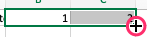
\includegraphics[scale=.4]{./images/tableur/recopieIncrementale_Excel_crop}, cliquer et tirer (en maintenant cliqué) vers la droite pour remplir les cellules suivantes jusqu'à la valeur 8 (voir image ci-dessous).
\end{itemize}

\uneimageici{./images/tableur/recopieIncrementale_Excel2_crop}{\textwidth}

\begin{itemize}
\item Cliquer dans la cellule \texttt{A2} et écrire \texttt{note sur 20}.
\item Remplir les cellules de la ligne 2 avec les notes correspondant aux différents tests.
\end{itemize}





\subsubsection{Sauvegarder le fichier}
\label{ssec_sauvegarder_fichier}
Il est important de sauvegarder régulièrement le fichier sur lequel on travaille. Sur la version en ligne d'\emph{Excel}, cela se fait automatiquement à partir du moment où le fichier a été enregistré une première fois.


Pour enregistrer votre travail sur la version logicielle d'\emph{Excel} :
\begin{itemize}
\item Ouvrir le menu \texttt{Fichier}.
\item Choisir \texttt{Enregistrer sous...}
\item Entrer le nom du fichier sous la forme \texttt{Nom-date}. \circled{1} comme dans l'exemple ci-dessous
\item Cliquer sur \texttt{Sur mon Mac} pour choisir où enregistrer le fichier. Cela transforme la fenêtre. \circled{2}
\item Choisir comme emplacement le \emph{Bureau} de l'ordinateur. \circled{3}
\item Vérifier que le fichier est bien enregistré au format \emph{Classeur Excel (.xlsx)}. \circled{4}
\end{itemize}

\uneimageici{./images/tableur/CalcEnregistrerFichier_Excel1_crop}{.7\textwidth}

\uneimageici{./images/tableur/CalcEnregistrerFichier_Excel2_crop}{.9\textwidth}

Une fois cela fait, appuyer régulièrement sur la combinaison de touche \texttt{cmd} + \texttt{S} : c'est le \emph{raccourci clavier} permettant d'enregistrer votre travail.

\uneimageici{./images/generales/clavierCmdS}{.5\textwidth}



\cadre{\textbf{Différence entre \texttt{Enregistrer} et \texttt{Enregistrer sous...}}\newline Dans la plupart des logiciels, on peut : \begin{itemize}\item \textbf{Enregistrer} le fichier sur lequel on travaille. Cette opération est possible si le fichier existe déjà et possède un nom. La version courante du fichier sera alors sauvegardée et remplacera l'ancienne version du fichier.
\item \textbf{Enregistrer sous...} le fichier sur lequel on travaille. Cette opération commence par demander un nouveau nom pour l'enregistrement du fichier. On peut donc ouvrir un fichier que l'on ne souhaite pas modifier, choisir \emph{enregistrer sous}, donner un nouveau nom et ainsi travailler sur une copie du fichier de départ.
%\item utiliser \texttt{cmd + s} (\emph{s} pour \emph{Save}) pour \textbf{enregistrer} le fichier courant. Bien que les documents soient enregistrés automatiquement par la majorité des logiciels, il faut régulièrement sauver son travail pour éviter les surprises.
\end{itemize}}









\subsubsection{Créer un graphique}\index{Calc!Créer un graphique}\index{Créer un graphique (Calc)}

\begin{itemize}
\item Sélectionner les données à représenter : cliquer sur la cellule \texttt{B1} sans relâcher le bouton et tirer (en maintenant cliqué) jusqu'à la cellule \texttt{I2}. Les cellules sélectionnées apparaissent en gris.
\uneimageici{./images/tableur/CalcCellulesSelectionnees_Excel_crop}{.9\textwidth}

\item Cliquer alors sur l'onglet \texttt{Insertion}\circled{1} puis sur la flèche à côté des icônes de graphiques pour voir la liste de tous les types de graphiques disponibles \circled{2}. Cliquez enfin sur l'image représentant le type de graphique souhaité. Dans notre cas, ce sera un graphique en nuage de points. \circled{3}
\uneimageici{./images/tableur/CalcBoiteDiagramme1_oExcel_crop}{.9\textwidth}
\end{itemize}

Vous avez maintenant un graphique qui s'est ajouté dans la feuille de calcul. Attention, la fenêtre du graphique est sélectionnée, ce qui est visible grâce aux huit poignées de sélection qui entourent la fenêtre :

\uneimageici{./images/tableur/CalcFenetreGraphiqueSelectionnee_oExcel_crop}{.6\textwidth}

Pour déplacer la fenêtre graphique, déplacer la souris sur le bord pour qu'apparaisse sur le curseur une croix. Le déplacement s'effectue en maintenant cliqué et en déplaçant la souris. Pour revenir à la feuille de calcul, cliquer sur n'importe quelle cellule (les poignées de sélection disparaissent alors).\\


Pour ajouter des titres aux axes, il faut d'abord sélectionner le graphique (à nouveau, vérifiez que les poignées de sélection sont bien présentes autour de celui-ci) et dans l'onglet \texttt{Graphique} cliquer sur \texttt{Titres des axes}  \circled{1}. Choisir ensuite l'axe pour lequel on veut ajouter un titre (exemple ici : l'axe horizontal : \circled{2}) et enfin l'option pour faire apparaitre un titre \circled{3}.

\uneimageici{./images/tableur/Calc_office_ajouter_titres_axes_crop}{.6\textwidth}

Une fenêtre s'ouvre alors, vous demandant d'écrire le titre qui va ensuite apparaître. Cliquez sur \texttt{OK} lorsque le titre vous convient.

Pour modifier le titre d'un axe ou le supprimer, les options pour ce faire apparaissent au même endroit où on a cliqué pour ajouter un axe, mais il faut choisir les options \texttt{Modifier le titre de l'axe horizontal...} (ou vertical) ou \texttt{Aucun} à la place de celle qui a ajouté un titre.


\subsubsection{Calculer la moyenne}\index{Moyenne (calcul de la)}\index{Calc!Moyenne (calcul de la)}

\begin{itemize}
\item cliquer dans la cellule \texttt{A4} et entrer le texte : \texttt{Moyenne}. \circled{1}
\item cliquer dans la cellule \texttt{B4} dans laquelle nous allons entrer une formule : \circled{2}
        \begin{itemize}
        \item taper un signe \texttt{=} qui signifie que la cellule va contenir une formule ;
        \item taper le nom de la formule suivie d'une parenthèse ouvrante : \texttt{=MOYENNE(} ;
        \item à l'aide de la souris, sélectionner dans la feuille de calcul les cellules contenant les notes dont on veut calculer la moyenne (voir image ci-dessous \circled{3}) ;
        \uneimageici{./images/tableur/CalcCalculMoyenne_Excel_crop}{.8\textwidth}
        \item appuyer sur la touche \texttt{Entrée} : la moyenne calculée apparaît.
        \end{itemize}
\end{itemize}



\subsubsection{Exporter au format PDF}\index{Calc!Exporter au format PDF}\index{PDF (exporter au format) (Calc)}

Une fois le travail achevé et sauvegardé, il faut exporter le fichier au format PDF. Pour cela, il faut passer par le menu \texttt{Fichier} et choisir \texttt{Imprimer} \circled{1} puis \texttt{Imprimer} \circled{2} comme si vous vouliez imprimer votre fichier.

\uneimageici{./images/tableur/Exporter_PDF_office_1_crop}{.4\textwidth}

S'ouvre alors un aperçu de votre document avec, à droite, quelques paramètres qui permettent notamment de changer l'échelle ou l'orientation de la page. Nous n'allons pas toucher à ces options et simplement nous contenter de cliquer sur le bouton \texttt{Impression}, en bas.

\uneimageici{./images/tableur/Exporter_PDF_office_2_crop}{.4\textwidth}

Il se peut que l'on vous demande une confirmation : dites alors que vous êtes sûrs que la page doit bien être imprimée. Vous allez voir c'est à cette étape que nous allons indiquer qu'il faut en réalité exporter le document au format PDF.

Dans la fenêtre qui apparaît, qui permet habituellement, de communiquer les réglages à l'imprimante, cliquer sur le bouton \texttt{PDF}, en bas à gauche. \circled{1} Parmi les options qui apparaissent, sélectionner \texttt{Enregistrer au format PDF}. \circled{2}

\uneimageici{./images/tableur/Exporter_PDF_office_3_crop}{.4\textwidth}

Vous pouvez ensuite choisir où vous désirez exporter votre nouveau fichier PDF. Faites attention à vous souvenir de l'endroit où vous l'enregistrez, car vous allez en avoir besoin plus tard.

\cadre{Le \textbf{format PDF} est un format parfaitement adapté aux échanges de documents : il est non modifiable et lisible sur tous les périphériques (ordinateurs, tablettes, smartphones). Il peut contenir du texte, des images, des liens vers l'internet et même des vidéos ou du son. \newline À chaque fois qu'il faut rendre ou envoyer un document qui n'est pas destiné à être modifié, il faut privilégier le format de fichier PDF.}

Sur l'application \emph{Excel}, il est également possible de n'exporter qu'un graphique au format PDF. Dans ce cas, il faut cliquer une fois sur le graphique puis cliquer droit dessus et choisir \texttt{Enregistrer en tant qu'image...}. S'ouvre alors la fenêtre ci-dessous.

\uneimageici{./images/tableur/Exporter_graphique_PDF_crop}{.7\textwidth}

En bas, sélectionnez le type de fichier souhaité (PDF). \circled{1} Cela met à jour l'extension du fichier dans la barre en haut de la fenêtre. \circled{2} Pour le reste, cela fonctionne de la même manière que précédemment.



\subsubsection{Remettre le travail achevé sur Teams}

Une fois le travail terminé et exporté au format PDF, il faut le remettre au professeur. Pour cela, se connecter à \emph{Teams} et accéder à l'équipe du cours. Cliquer sur \texttt{Devoirs} et cliquez sur le devoir correspondant à l'activité que vous êtes en train de terminer. Cliquez sur \texttt{Ajouter un travail}, en bas, puis \texttt{Charger à partir de cet appareil}, en bas à gauche. Sélectionnez le fichier au format PDF que vous venez d'exporter et \texttt{Ouvrir}. Une fois le travail chargé, cliquez sur \texttt{Terminé}, en bas à droite. Enfin, cliquez sur \texttt{Remettre}, en haut à droite.\\



Si nécessaire, se reporter à la fiche méthode \emph{Remettre un devoir sur Teams}, page \pageref{TeamsRemettreDevoir}.



